\documentclass[10pt,a4paper,oneside,fleqn]{article}
\usepackage[slovene]{babel}     % za prikaz šumnikov
\usepackage[utf8]{inputenc}     % za prikaz šumnikov
\usepackage{amsfonts}           % doda zbirko matematičnih znakov
\usepackage{graphicx}           % prikaz slik
\usepackage{longtable}          % paket za tabele, ki se raztezajo čez več strani
\usepackage{subcaption}

% Nastavitve strani
\setlength{\oddsidemargin}{-0. cm} 
\setlength{\evensidemargin}{-0. cm}
\setlength{\topmargin}{-0.54 cm}   
\setlength{\textwidth}{16. cm}     
\setlength{\textheight}{24 cm}     
\setlength{\marginparsep}{3 mm}    
\setlength{\marginparwidth}{1.5 cm}

% Nastavitve odstavka
\setlength{\parindent}{0 mm}       
\setlength{\parskip}{1.5ex plus 0.5ex minus 0.5ex}
\renewcommand{\baselinestretch}{1.25}
\setlength{\mathindent}{1 cm}      

% Literatura
\bibliographystyle{unsrt}		% literatura je sortirana po vrstnem redu prve navedbe

% Kazalo
\setcounter{tocdepth}{2}

% Povezave, aktiven dokument
\usepackage[unicode]{hyperref}		% naredi dokument aktiven (v DVI in PDF) -> mora biti vedno zadnji pred začetkom dokumenta
%%%%%%%%%%%%%%%%%%%%%%%%%%%%%%%%%%%%%%%%%%%%%%%%%%%%%%%%%%%%%%%%%%%%%%%%%%%%%%%%%%%%%%%%%%%%%%%%%%%%
% sedaj začnemo dokument
\begin{document}
	
	
	\begin{center}
		REPORT
		
		Jure Cej\\
		2023-02-09
	\end{center}


Axisimetrical FEM simulation of O-ring with 3,5mm diameter and 4mm in a groove of 3,1 mm.



O-rings properties and dimensions.

Material: EPDM 70 ShA \\
$d_1 =$ 3,5 mm O-ring 1 diameter\\
$d_2 =$ 4 mm O-ring 2 diameter\\
$D =$ 90 mm inner O-ring diameter\\
$E =$ 4,5 MPa\\
$\nu =$ 0,3 \\
$\rho = $ 1,14$\cdot10^{-9}$ ton/mm$^3$ \\
$t =$ 1 s


\begin{figure}[h]
	\centering
	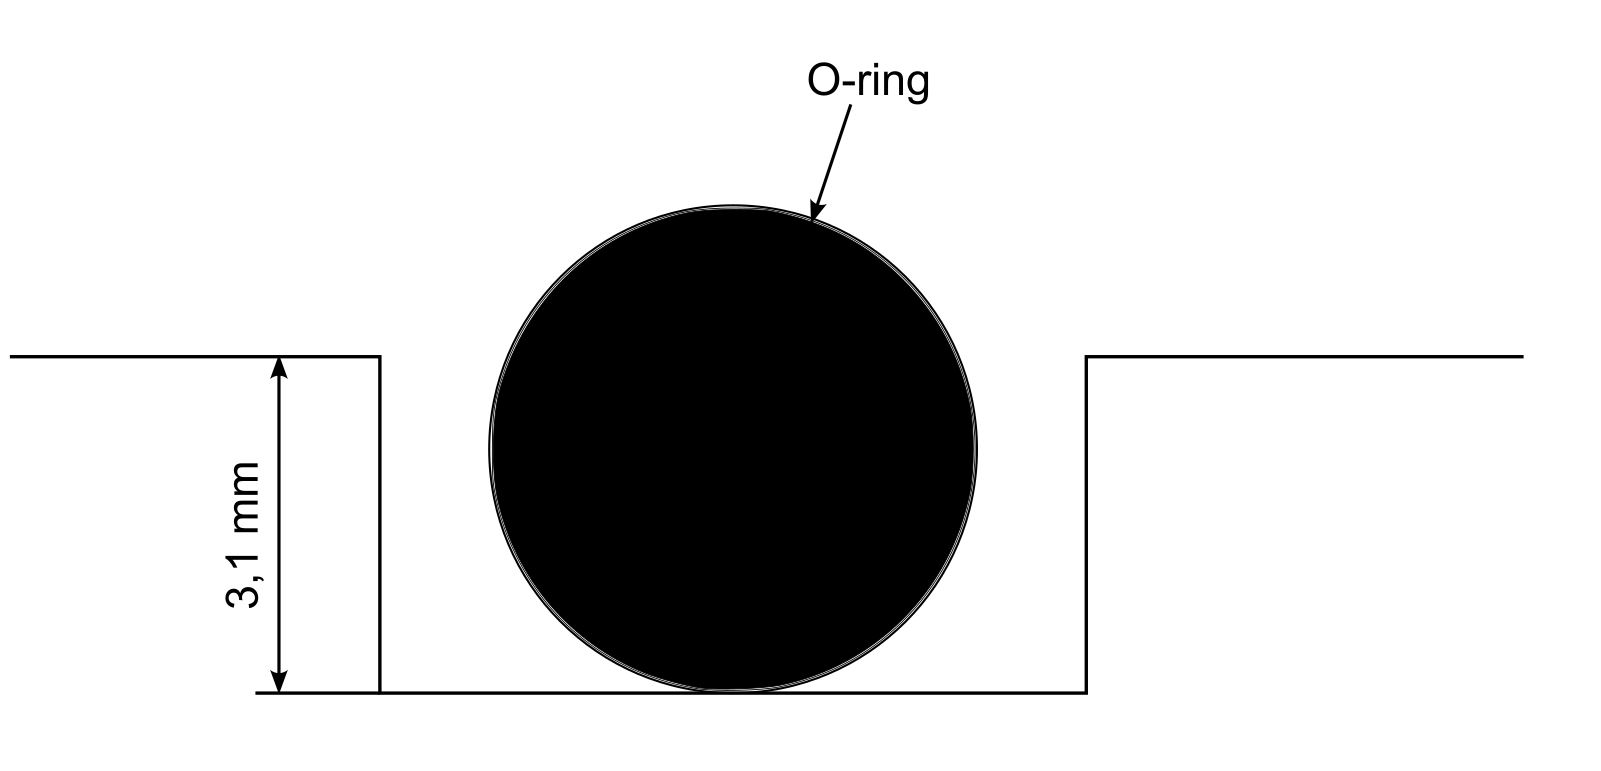
\includegraphics[width=0.5\textwidth]{2023-02-09-O-ring}
	\caption{O-ring in groove.}
	\label{fig:2023-02-09-O-ring}
\end{figure}



\begin{figure}[h]
	\begin{subfigure}{0.55\textwidth}
		\centering
		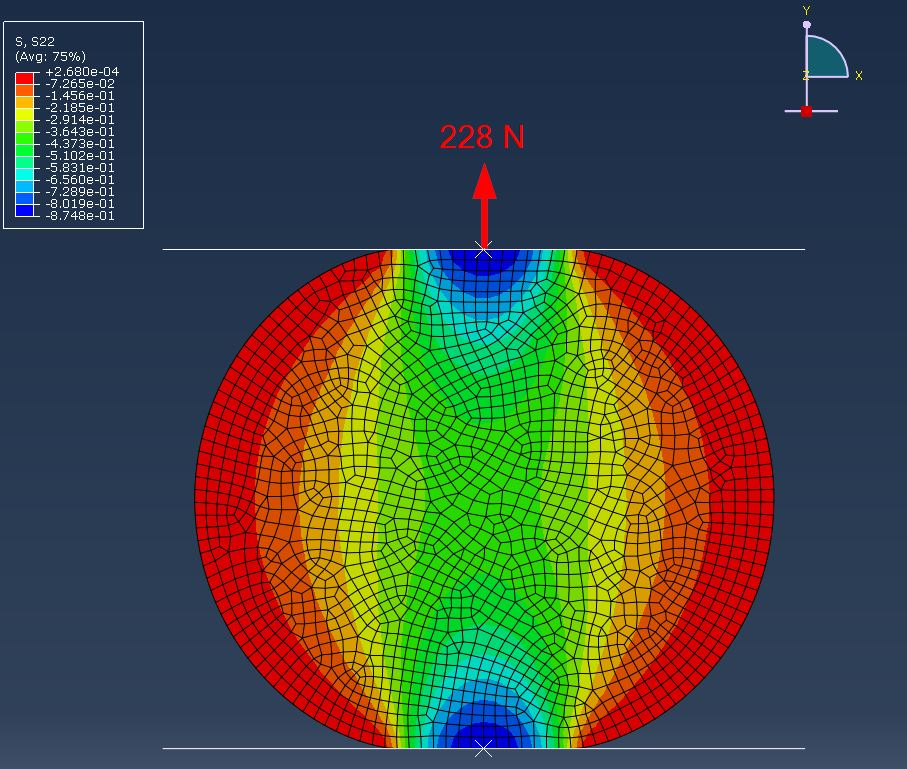
\includegraphics[width=1\textwidth]{2023-02-09-3mm5}
		\caption{O-ring $d=$ 3,5 mm.}
		\label{fig:2023-02-09-3mm5}
	\end{subfigure}
	\begin{subfigure}{0.45\textwidth}
		\centering
		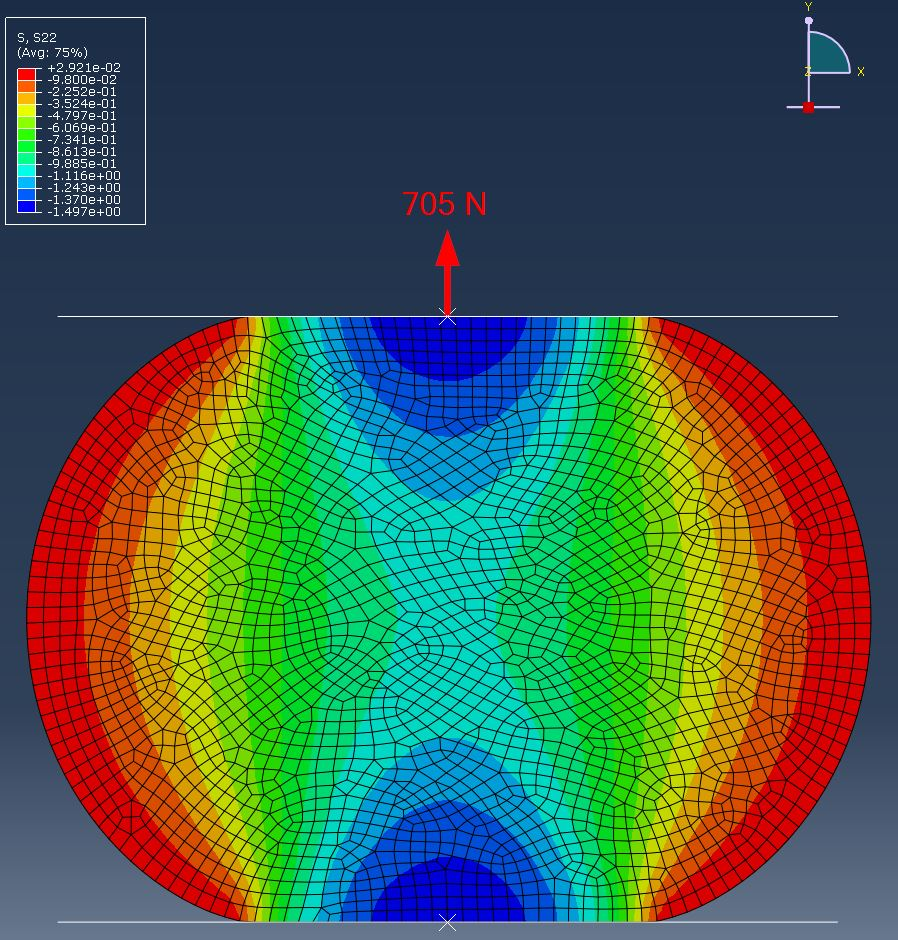
\includegraphics[width=1\textwidth]{2023-02-09-4mm}
		\caption{O-ring $d=$ 4 mm.}
		\label{fig:2023-02-09-4mm}
	\end{subfigure}
\end{figure}


\end{document} 